\documentclass{standalone}
\usepackage{tikz}
\usepackage{pgfplots}
\pgfplotsset{compat=1.12,width=5cm}%
\begin{document}
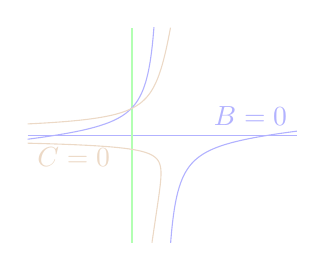
\begin{tikzpicture}
\newcommand{\mx}{4}
\newcommand{\lamb}{-.1}
\begin{axis}[hide axis,xmin=-\mx,xmax=\mx,ymin=-\mx,ymax=\mx]
\newcommand{\fclr}{blue!30}
\draw[\fclr] 
	(-\mx,0) 
-- (\mx,0) node[above left]{\(B=0\)};
\newcommand{\gclr}{brown!30}
\draw[green!30] ({-(\lamb+1)},-\mx) -- ({-(\lamb+1)},\mx);
  \addplot[domain=-\mx:-.1,\fclr,samples=200]{-\lamb*x-1/x};%
  \addplot[domain=.1:\mx,\fclr,samples=200]{-\lamb*x-1/x};%
  \addplot[domain=.1:\mx,\gclr,samples=200]({-(2*\lamb*x^3+x+1)/(2*x^2)},{x});
  \addplot[domain=-\mx:-.1,\gclr,samples=200]({-(2*\lamb*x^3+x+1)/(2*x^2)},{x});
    \node[\gclr,below right] at (-\mx,-.1) {\(C=0\)};
\end{axis}
\end{tikzpicture}
\end{document}
